% boavizta mention immaturity of assessments and variability of estimates

\documentclass[11pt]{article}
\usepackage[margin=0.9in]{geometry}
\usepackage[T1]{fontenc}
\usepackage{libertine}
\renewcommand{\sfdefault}{fvs} % Use as sans-serif
\renewcommand{\ttdefault}{fvm} % Use as monospace
\renewcommand{\ttfamily}{\small\fontfamily{\ttdefault}\selectfont} % Slightly smaller monospace font
\newcommand{\eg}{{\em e.g.}}
\newcommand{\coe}{CO$_2$e}
\newcommand{\gcoe}{g \coe}
\newcommand{\tcoe}{t \coe}
\newcommand{\kgcoe}{k\gcoe}
\newcommand{\gcoekwh}{\gcoe\ / kWh}
%\usepackage{helvet} % Helvetica font for sans-serif
%\usepackage{courier} % Courier font for monospace
\usepackage{graphicx}
\usepackage{hyperref}
\hypersetup{
    hidelinks
}
\usepackage[style=numeric]{biblatex}
\usepackage{titlesec}
\usepackage{enumitem}
\usepackage{titling}

\titleformat{\section}{\sffamily\Large}{\thesection}{1em}{}
\titleformat{\subsection}{\sffamily\large}{\thesubsection}{1em}{}
\titleformat{\subsubsection}{\sffamily\normalsize}{\thesubsubsection}{1em}{}
\setlength{\parindent}{0pt}
\setlength{\parskip}{0.5em}

\addbibresource{ref.bib}
\title{Modeling the impact of IT- and AI-related emissions in a university setting}
\author{Massimiliano Poletto\thanks{Independent consultant, max.poletto@gmail.com}, Nils Handler\thanks{University of Zürich, nils.handler@uzh.ch. Contact author.}}

\begin{document}

\maketitle

\section*{Abstract}
Information technology (IT) plays a major role in society and has non-negligible environmental impact, accounting for over 5\% of global electricity consumption and about 2\% of global carbon emissions. Moreover, artificial intelligence (AI) applications, especially large language models (LLMs), are being adopted at historically high rates. Their growth is expected to increase the share of global electricity consumption for data centers from $\sim 1\%$ in 2024 to $\sim 3\%$ by 2030. Therefore, an assessment of IT and AI emissions is a necessary component of any net-zero roadmap. As part of the University of Zürich's own net-zero efforts, we have attempted to quantify and analyze the impact of IT and AI on the university's carbon footprint. We present a simple interactive model of IT emissions on a university campus. The model approximates operational and lifecycle emissions of personal devices, university-owned computing and network infrastructure, cloud computing, and LLMs. The model is intended to provide university decision makers with emissions estimates under different scenarios, with sufficient accuracy to support effective decision-making. Our analysis shows that the embodied emissions of IT infrastructure and personal devices are a major component of overall IT emissions, that operational impacts are comparatively modest, and that LLM adoption, even under aggressive growth scenarios, is unlikely to comprise more than $5\%$ of overall IT-related emissions.

\section{Introduction}

Information technology accounts for over 5\% of global electricity consumption and at least 1.7\% of global carbon emissions~\cite{wb:itu:ict}. At the University of Zürich (UZH), which with over 38,000 students and staff is the largest Swiss university, IT in 2024 accounted for about 1.5 M\tcoe\ (megatons of carbon dioxide equivalent) of greenhouse gas (GHG) emissions, approximately 6.3\% of total university emissions in 2024~\cite{uzh:sustainability:report}. The cited report takes into account university-owned workstations, servers, and audiovisual equipment, but does include other IT-related activities such as networking, cloud computing, or the growing use of artificial intelligence, and in particular the adoption of generative AI and large language models (LLMs).

AI applications are being adopted at historically high rates, more quickly than the personal computer or the internet were adopted in the past~\cite{bick:ai:adoption}. Enterprise AI adoption has accelerated, with generative AI tools seeing widespread deployment across industries within months of their release~\cite{mckinsey2024ai}. In July 2025, ChatGPT received 2.5 billion queries per day, up from 1 billion in December 2024, and within an order of magnitude of Google's approximately 15 billion queries per day~\cite{techcrunch:chatgpt}. AI growth is currently projected to increase the share of global electricity consumption for data centers from $\sim 1\%$ in 2024 to $\sim 3\%$ by 2030~\cite{iea:ai:energy}.

The University of Zürich has set itself the target of becoming climate-neutral by 2030 within the categories of energy, transportation, food, and waste, with additional goals in 2035 and beyond~\cite{uzh:sustainability:report}. Given the current sizable contribution of IT to the university's emissions, and the potential for growth through AI adoption in the coming years, we felt it was necessary to understand IT emissions and their growth trajectories in more detail.

This paper presents a simple interactive model of IT emissions on a university campus. We developed it in the specific context of the University of Zürich, but believe that it is parameterizable and general enough to apply to other similar university campuses or large corporate facilities.

We seek to answer three broad questions:
\begin{itemize}
  \item What are the main contributors to the IT emissions of a university?
  \item Could migrating some on-campus IT services to commercial cloud providers decrease the overall campus footprint?
  \item What is the likely impact of the surge in AI adoption? In particular, will the emissions impact of AI be so large as to make other sources of IT emissions negligible?
\end{itemize}

Our model sets relatively broad system boundaries. It takes into account university-owned equipment but also university services hosted by commercial cloud providers and university use of commercial generative AI products. We have also parameterized it to account for student devices not owned by the university, since they are key to student work and constitute the bulk of the university's end-user devices. We attempt to model devices' full lifecycle impact, including manufacture and disposal. 

Experts rightly point to the many potential benefits of AI in the areas of climate change mitigation and adapation~\cite{climate:change:ai}. On a university campus, these might include more efficient building heating and cooling, improved transportation logistics, etc. However, those benefits are still to come and difficult to predict. In this paper, we consider only the {\em direct} impacts of AI in terms of increased electricity consumption and the resulting emissions.

The rest of this paper is organized as follows. Section~\ref{sec:model:methodology} presents the general modeling framework, including system boundaries and assumptions. Section~\ref{sec:model:details} justifies some of the specific parameter values used in the model. Section~\ref{sec:results} describes results and explores different scenarios and assumptions. Section~\ref{sec:recommendations} offers recommendations to university IT administrators. Section~\ref{sec:related:work} describes related work in this area.

\section{Modeling methodology}
\label{sec:model:methodology}

Our aim is to model energy use from university IT and AI broadly, without restricting ourselves to university-owned devices, specific IT departments, etc. At the same time, we want to be able to distinguish the contributions of different factors, such as student-owned devices or LLMs, and to compare the model's output against existing university data points (energy bills, etc.).

\subsection{System boundaries}

We define the boundaries of our model as follows.

\subsubsection*{Population}

We include IT-related activity from all members of the UZH community: faculty, staff, and students.

\subsubsection*{On-campus devices}

Student-owned devices, such as laptops and smartphones, are in scope, since they are the primary means by which students access university IT services and do their coursework. Given the duration of studies, we include personal devices' embodied emissions in the model.

University-owned devices are in scope. We have accurate numbers for staff workstations, classroom computers, network access points, and audiovisual devices managed by the central IT department. We can only estimate other devices, such as networking equipment or computers managed by individual research groups. As before, we include these devices' embodied emissions in the model.

For servers, which are mostly located in on-premise data centers, we also attempt to take into account emissions from cooling. (We do not model the manufacturing emissions of the cooling equipment itself.)

\subsubsection*{Cloud and supercomputing facilities}

UZH at present does not make significant use of commercial cloud compute, but the model allows simulating the shift of some fraction of the server load to cloud VMs. For this hypothetical cloud footprint, like for on-premise data centers, we attempt to model operational emissions, embodied emissions, and emissions from cooling.

UZH faculties do use shared off-campus supercomputing facilities, primarily the Swiss National Supercomputing Center, CSCS~\cite{cscs}. We estimate the operational impact of these workloads, but, due to lack of data, we do not include embodied emissions or cooling. This omission undercounts total university IT energy use but overestimates the potential relative impact of AI.

Due to lack of data, we do not model emissions from application-level cloud services such as Microsoft 365 or Google Workspace. Again, this undercounts total IT energy use but overestimate the relative impact of AI.

\subsubsection*{Large language models}

We estimate inference-time emissions of current large language models based on the literature. We also include training-time emissions, embodied emissions, and likely cooling overhead of language models (these are harder to measure and we err on the side of overestimating them).

\subsubsection*{Summary}

This table summarizes what is in scope in the current model. The main gap is emissions of cloud services such as Microsoft 365 or Goole Workspace.

\begin{center}
  \begin{tabular}{|l|c|c|c|}
    \hline
    \textbf{Device or service} & \textbf{Operation} & \textbf{Lifecycle} & \textbf{Cooling} \\ \hline
    Student laptops \& phones & yes & yes & n/a \\
    University workstations, access points, etc. & yes & yes & n/a \\
    University on-premise servers & yes & yes & yes \\
    Cloud servers & yes & yes & yes \\
    Cloud services & no & no & no \\
    Supercomputing facilities & yes & no & no \\
    LLMs & yes & yes & yes \\ \hline
  \end{tabular}
  \label{tab:scopes}
\end{center}

\subsection{Accounting approach}

\subsubsection*{On-campus devices}

We model campus device emissions bottom-up. We first identify categories of devices (phones, laptops, workstations, monitors, routers, etc.). For each device type, we research a range of common models, then use manufacturer data sheets or other available documentation to identify operational power draw (in watts) as well as embodied emissions related to manufacture and disposal (in \kgcoe) per device. Based on this data, we model the power draw and embodied emissions of an ``exemplar'' device of each type.

For each device type we also estimate (1) a count (\eg, a laptop for every student and staff), (2) an estimated duty cycle (\eg, laptops used 8 hours per day, 200 days per year), and (3) a useful lifetime (in years).

Given all this, for each device type we can straightforwardly obtain an annual energy use (kWh) and annual embodied emissions (embodied emissions amortized over useful lifetime) (\kgcoe). We then estimate the local grid's carbon emissions intensity (\gcoekwh) to convert the energy use to emissions and obtain a combined total annual emissions number\footnote{The model can also operate stochastically, instantiating devices from a distribution, but we lack good data on the  form of such a distribution, so we limit our analysis to this simple linear mode.}.

The Swiss Federal Office for the Environment has an extensive report on the environmental impact of electricity generation in Switzerland~\cite{krebs2018umweltbilanz}, but we are fortunate to also have hourly emissions intensity data from \textcite{electricitymaps}. We use the hourly intensity data for {\em consumption} (not production) to compute emissions intensity for every hour of the day averaged over all days in 2024. Emissions vary from a high of 64 \gcoekwh\ in the middle of the night to a low of 45 \gcoekwh\ in the middle of the day. This variation is sufficiently large that we refine the model's device duty cycle to represent four six-hour periods over the course of the day. It allows us to specify, for example, that user devices are mostly used during the day whereas servers run around the clock.

For servers (in on-premise data centers) we also account for cooling overhead. Based on limited UZH historical power data, we estimate that the on-premise power usage effectiveness (PUE), the ratio of total data center power (including cooling) to power used for computation, is approxmiately 2. This value, higher than the commercial average of 1.56~\cite{google:datacenter:efficiency}, is attributable to inefficient cooling.

\subsubsection*{Cloud and supercomputing facilities}

We attempt to model a hypothetical shift of some workloads from servers in an on-premise data center to a commercial cloud. We model the shift as a fraction of servers that are moved to the cloud, the average conversion ratio of on-premise servers to cloud servers, and cloud data center PUE and electricity emissions intensity (since the cloud data center may be located in a different region than the on-premise data center).

As mentioned earlier, we do not attempt to model application-level cloud services.

For supercomputing facilities (in particular, CSCS) we rely on annual statistics of total power consumption for peak compute load and make assumptions about duty cycle. We do not have reliable data about the embodied emissions of the facility, but suspect that the fraction of these emissions that is attributable to UZH use is negligible relative to all other UZH emissions.

\subsubsection*{Large language models}

For LLMs, we estimate operational energy use (Wh per query) using current estimates in the literature of state-of-the-art models~\cite{devries2023growing,epoch2025howmuchenergydoeschatgptuse}.

We consider the training overhead and the embodied emissions of the servers and GPUs that the model runs as a fixed cost that is amortized across all queries to a model. As a result, in practice, this overhead is constantly shrinking. We incorporate it into the model as a configurable percentage overhead of the operational energy use.

\section{Model details}
\label{sec:model:details}

The previous section describes our overall modeling approach, which we believe is broadly applicable to university and other large campus settings. This section presents the reasoning behind specific values we employ in the UZH evaluation.

\subsection{On-campus devices}

\subsubsection*{Number of devices}

We have an authoritative census of devices (workstations, servers, audiovisual equipment) managed by central IT, as follows.

\begin{center}
  \begin{tabular}{|l|r|r|}
    \hline
    \textbf{Device type} & \textbf{Count} & \textbf{Life (y)}\\ \hline
    Laptops & 10,440 & 4 \\
    Monitors & 10,400 & 6 \\
    Servers & 1,121 & 5 \\
    Printers & 333 & 6 \\
    Mobile phones & 2,439 & 3 \\
    A/V devices & 431 & 6 \\ \hline
  \end{tabular}
  \label{tab:oncampusdevices}
\end{center}

In addition to these numbers, which cover staff and facilities, we assume that 80\% of the student population of 28,000 people have a laptop (or equivalent device, such as a tablet), and that everyone at the university has mobile phone, resulting in a rough estimate of 32,000 laptops and 35,000 mobile phones.

Traditional desktop computers appear to be infrequent on campus. By default we set their number to zero in our model, but we still provide the framework to model them if desired.

\subsubsection*{Operational emissions}

The Swiss electricity mix is substantially cleaner than the European or North American average, so generic manufacturer estimates of lifetime usage-related emissions are unsuitable. Unfortunately, in manufacturer documentation we found surprisingly few sources of data on device power consumption, as opposed to estimated lifetime CO$_2$ emissions. Based on some manufacturer data sheets, primarily from Apple, Cisco, and Dell, we model power draw of different devices while under load using the following initial parameters:

\begin{center}
  \begin{tabular}{|l|r|r|}
    \hline
    \textbf{Device} & \textbf{Mean (W)} & \textbf{$\sigma$ (W)} \\ \hline
    Laptop & 30 & 5 \\ \hline
    Monitor & 50 & 10 \\ \hline
    Desktop & 100 & 20 \\ \hline
    Server & 400 & 100 \\ \hline
    Mobile phone & 5 & 2 \\ \hline
    A/V equipment & 250 & 50 \\ \hline
    Printer & 1000 & 200 \\ \hline
  \end{tabular}
\end{center}

Our assumptions about device duty cycle can be summarized as follows: (1) end-user devices are used during the day on weekdays, (2) servers run around-the-clock but at 80\% of peak power load, (3) mobile phones draw no power (they are unplugged) except for a few hours in the evening to charge, (4) printers are idle except for a few minutes per day. Standby power for all devices is negligible ($\sim 1$ W), except for printers which often draw 50--100 W.

We lack good data about the campus network, save for the existence of approximately 4,000 wifi access points. Based on this, we choose to model network emissions as a configurable percentage of device (local, desktop, server) emissions, by default 10\%.

\subsubsection*{Embodied emissions}

For several device types, especially end-user devices such as phones and laptops, embodied emissions
comprise a majority of lifetime emissions. Different sources report widely different values for these emissions. Our approach has been to find several studies and industry references, and then estimate a mean reference value as well as likely minimum and maximum values.

The following table summarizes results from the literature.

\begin{center}
  \begin{tabular}{|l|r|l|}
    \hline
    & \textbf{Embod. emiss.} & \\
    \textbf{Device type} & \textbf{(\kgcoe)} & \textbf{Source} \\ \hline
    Laptop & 121 & \textcite{ecoinvent}  \\ \hline
    Laptop & 104 & \textcite{teehan2013} (low) \\ \hline
    Laptop & 338 & \textcite{teehan2013} (high) \\ \hline
    Laptop & 244 & \textcite{rarecoil} \\ \hline
    Laptop & 202 & \textcite{unctadder2024} \\ \hline
    Desktop & 238 & \textcite{ecoinvent} \\ \hline
    Desktop & 303 & \textcite{teehan2013} \\ \hline
    Desktop & 403 & \textcite{unctadder2024} \\ \hline
    Desktop & 289 & \textcite{dellpcf} \\ \hline
    Desktop & 277 & \textcite{boavizta:api} \\ \hline
    Server & 383 & \textcite{teehan2013} \\ \hline
    Server & 1252 & \textcite{davy2021} (Dell) \\ \hline
    Server & 1912 & \textcite{davy2021} (EC2) \\ \hline
    Server & 899 & \textcite{boavizta:api} (medium server)\\ \hline
    Phone & 68 & \textcite{googlepixel8} (Pixel 8)\\ \hline
    Phone & 54 & \textcite{appleiphone13} (iPhone 13)\\ \hline
    Phone & 50 & \textcite{unctadder2024} \\ \hline
    Phone & 50 & \textcite{lovehagen2023} \\ \hline
    \end{tabular}
  \label{tab:embodied_emissions}
\end{center}

For laptops, the numbers from Ecoinvent, a reputable proprietary Swiss life cycle inventory database used in the UZH sustainability report, appear to be on the low end. The most comprehensive publicly available data comes from \textcite{rarecoil}, which lists manufacturer information for over 90 popular devices. Mean supply chain emissions in this data set are 244 \kgcoe\ with a standard deviation of 128 kg. To be conservative, we split the difference between this number and the Ecoinvent values and model laptops embodied emissions at 180 \kgcoe\ / device.

For desktops, most estimates are in the range of 250 - 400 \kgcoe. The most detailed data comes from Dell's Product Carbon Footprints (\cite{dellpcf}), which the company publishes for each of their products. A sample of 15 desktops has mean supply chain emissions of 289 \kgcoe\ with $\sigma = 80$ kg. We model desktop embodied emissions at 290 \kgcoe\ / device.

In the case of servers, \textcite{davy2021} reports manufacturer data for many Dell servers and estimates for different types of EC2 instances. The former have mean supply chain emissions of 1252 \kgcoe\ with $\sigma = 330$ kg, the latter 1912 kg with $\sigma = 885$ kg. \textcite{boavizta:api} reports mean supply chain emissions of 899 \kgcoe\ for a medium-sized server. We model server supply chain emissions at 1100 \kgcoe\ / device.

The variability of estimates for mobile phones is much smaller. We model phone embodied emissions at 50 \kgcoe\ / device.

We found less data for other types of devices. For now, we model them as follows:

\begin{itemize}
  \item Computer monitors: 340 \kgcoe\ (\cite{teehan2013}, \cite{dellpcf}).
  \item Conference room displays: 700 \kgcoe\ (scaling monitor by $(40''/27'')^2$). We use this as a proxy for all audiovisual equipment (lecture room projectors, etc.). Note that the numbers are sufficiently low that errors in this estimate do not significantly affect the overall result.
  \item Printer/copier stations: 1100 \kgcoe\ (\cite{ecoinvent}).
  \item Network equipment: We did not find reliable lifecycle assessments for routers and switches, and have little information about UZH network architecture. The vast majority ($80-95\%$) of lifecycle emissions of network gear stem from usage (\cite{cisco2024}, \cite{jacob2023}). For now, we model the embodied emissions of network equipment like we do its operational emissions, namely as a 10\% overhead on the number of devices (laptops, desktops, servers).
\end{itemize}

\subsection{Cloud and supercomputing facilities}

The secretiveness of major cloud providers makes it difficult to estimate the embodied and operational emissions of cloud infrastructure. The best resource we have found is the Datavizta API by the Boavizta working group~\cite{boavizta:api}.

Lacking information about UZH's workloads, we model a hypothetical UZH cloud footprint as the replacement of one campus server with a configurable number (by default, one) of Azure {\tt standard\_d48s\_v3} instances (Intel Xeon, 48 cores, 192 GB RAM, 2TB SSD)~\cite{msftvms}. Based on data from Boavizta, such a machine has embodied emissions of 667 \kgcoe\ and mean electricity power usage of 255 W. Given the uncertainty, we round up to 700 \kgcoe\ and 255 W. We assume deployment to Microsoft Azure's ``\href{https://datacenters.microsoft.com/globe/explore?info=region_switzerlandnorth}{Switzerland North}'' region, which makes sense for a Swiss university and means that the electricity mix is the same as for on-premise facilities. We estimate a power usage effectiveness of 1.15 for this facility. (As of 2025, average PUE for cloud computing is 1.56, with Google averaging 1.09 across its fleet~\cite{google:datacenter:efficiency} and Microsoft ranging from 1.14 to 1.19 in Europe~\cite{microsoft:datacenter:efficiency}.)

Given all these parameters, we can then compute cloud server operational emissions, embodied emissions, and cooling overhead as we do for on-premise servers.

For supercomputing at CSCS, unfortunately, our only available data is power utilisation at peak load, 131 kW in 2024. We assume a 50\% average load and use the Swiss emissions intensity numbers to compute annual operational emissions.

\subsection{Large language models}

The energy consumption of LLMs is being studied extensively~\cite{budennyy2022eco2ai,castano2023exploring,devries2023growing,epoch2024optimallyallocatingcomputebetweeninferenceandtraining,gowda2024watt,harding2024watts,heguerte2023estimate,luccioni2022estimating,luccioni2023counting,patterson2021carbon,rodriguez2024evaluating,tripp2024measuring,epoch2025howmuchenergydoeschatgptuse}.

A widely cited 2023 study~\cite{devries2023growing} estimated the average energy consumption of a large language model like ChatGPT at approximately 3 Wh / request, about ten times the energy of a standard Google search query. In 2025, \textcite{epoch2025howmuchenergydoeschatgptuse} makes a convincing case that the energy use for the average GPT-4o query is now just 0.3 Wh, ten times smaller than the 2023 estimate, while admitting that for unusually long inputs (10K--100K tokens) or more ambitious applications such as OpenAI's Deep Research~\cite{oai:deepresearch} the energy requirement might rise into the tens of watt-hours.

Improvements in hardware technology and an increased focus on software optimization by AI companies as adoption of AI grows mean that, for a given level or quality of model, inference costs are likely to continue to drop rapidly. To be conservative, in the model we assume that queries consume 1 Wh each on average.

By contrast, due to the increasing size and complexity of state-of-the-art models, the power required to train such models has been doubling annually~\cite{epoch2024powerusagetrend}. The literature offers little insight into the relative electricity consumption of training and inference~\cite{verdecchia2023systematic}, but Google~\cite{patterson:footprint:2022} reports that in 2019--2021 inference accounted for about 60\% of AI energy consumption, implying a ratio of training energy to inference energy was 2:3.

Another way to estimate training overhead is to consider that training Llama 3.1, a model comparable to GPT-4o, required approximately 25 MW of power for three months, or 54 GWh. Assuming ChatGPT's recently reported 2.5 billion queries per day~\cite{techcrunch:chatgpt} and a conservative (for this analysis) 0.3 Wh per query, ChatGPT consumes 750 MWh / day. If the model is used for 9 months before being replaced, inference energy amounts to 203 GWh, so the ratio of training to inference is 54:204 $\approx$ 1:4. (Assuming 1 Wh per query, inference energy is 675 GWh, and the ratio is 1:13, making training overhead negligible.) To be conservative, in the model we assume a ratio of 1:4.

We must also examine embodied emissions. \textcite{epoch2025howmuchenergydoeschatgptuse} estimates 1 second of NVIDIA H100 GPU time per query. NVIDIA reports~\cite{nvidia:h100} a cradle-to-gate carbon footprint of 1,312 \kgcoe\ for one H100. GPUs are typically hosted in sets of 4 or 8 in servers such as the NVIDIA DGX~\cite{nvidia:dgx}. Assuming a high-end server footprint of 2,000 \kgcoe\ for such a device and dividing by 8 GPUs, we obtain 250 \kgcoe\ server overhead per GPU. If this platform is used for three years at 70\% efficiency, we straightforwardly obtain embodied emissions of 0.01 \gcoe\ per query.

% 3 * 365 * 24 * 3600 / .7 = 135154285 queries
% (1312+250)*1000 = 1562000 grams
% 1562000/135154285 grams / query

Finally, there is the question of electricity mix. The facilities hosting LLMs are distributed and the location that serves a particular request is unknown. To map energy use to emissions we use the average emissions intensity of electricity generation in the EU in 2023, 207 \gcoekwh~\cite{eea:emissions:2025}.

In summary, we make the following default assumptions:

\begin{itemize}
  \item LLM energy consumption of 1 Wh per query.
  \item Training overhead of 25\%. In other words, inference plus training amounts to 1.25 Wh per query.
  \item Carbon emission intensity of 207 \gcoekwh.
  \item Embodied emissions of 0.01 \gcoe\ / query.
\end{itemize}

Of course, we must also make assumptions about the fraction of the university population that use LLMs and the frequency of use (queries / day). By default we assume that the average every user will issue 15 queries per day.

\subsection{Model limitations}

Our biggest limitation is the relative lack of ground truth data about UZH IT infrastructure. We have obtained only estimates of campus data center energy use, and little information abut UZH research workloads (whether AI-related or not). We assume that many research AI workloads will be relatively similar in intensity to existing scientific computation workloads. We also lack information about UZH use of external high-performance compute resources at CSCS.

Additionally, our work relies on assumptions and anecdotal evidence about device ownership and use among the university population, use of generative AI tools, etc.

Moreover, cloud vendors and AI companies are secretive about their infrastructure, and we have had to rely on public datasets and research literature to estimate cloud and AI emissions.

However, all these points of uncertainty are exposed as user-configurable parameters in the model, allowing easy sensitivity analysis and exploration of alternate scenarios.

\section{Results}
\label{sec:results}

\subsection{Initial model validation}

Using only the types of devices reported in the UZH 2024 Sustainability Report~\cite{uzh:sustainability:report}, and restricting embodied emissions to the Ecoinvent~\cite{ecoinvent} model used by that report, our model estimates emissions of 1,460 \tcoe, within 1\% of the 1,454 estimated in the UZH report, even though the methodology is somewhat different. Our model exposes average device power ratings and duty cycle, grid emissions intensity, etc., directly, whereas the approach used in the sustainability report relies on gross emissions factors (\kgcoe\ / device for embodied emissions, \kgcoe\ / device / day for operational emissions) provided by Ecoinvent.

While this is admittedly just one data point, and the extreme proximity of the two values is likely a coincidence, it provides some confidence that our assumptions are reasonable and that the model can be used to make directional decisions and extrapolate trends beyond the immediate scope of the sustainability report.

\subsection{Key results}

We now discuss the main takeaways from our model when it is configured with the parameter values described above. In Section~\ref{sec:sensitivity:analysis} we explore how these results change under different assumptions.

\subsubsection*{Impact of embodied emissions}

Maybe the most striking result is that, when we consider the entire population of campus devices, and not only those owned and managed by the university, overall emissions are absolutely dominated by the manufacturing and disposal of end-user devices. See Figure~\ref{fig:1}.

\begin{figure}[h]
  \centering
  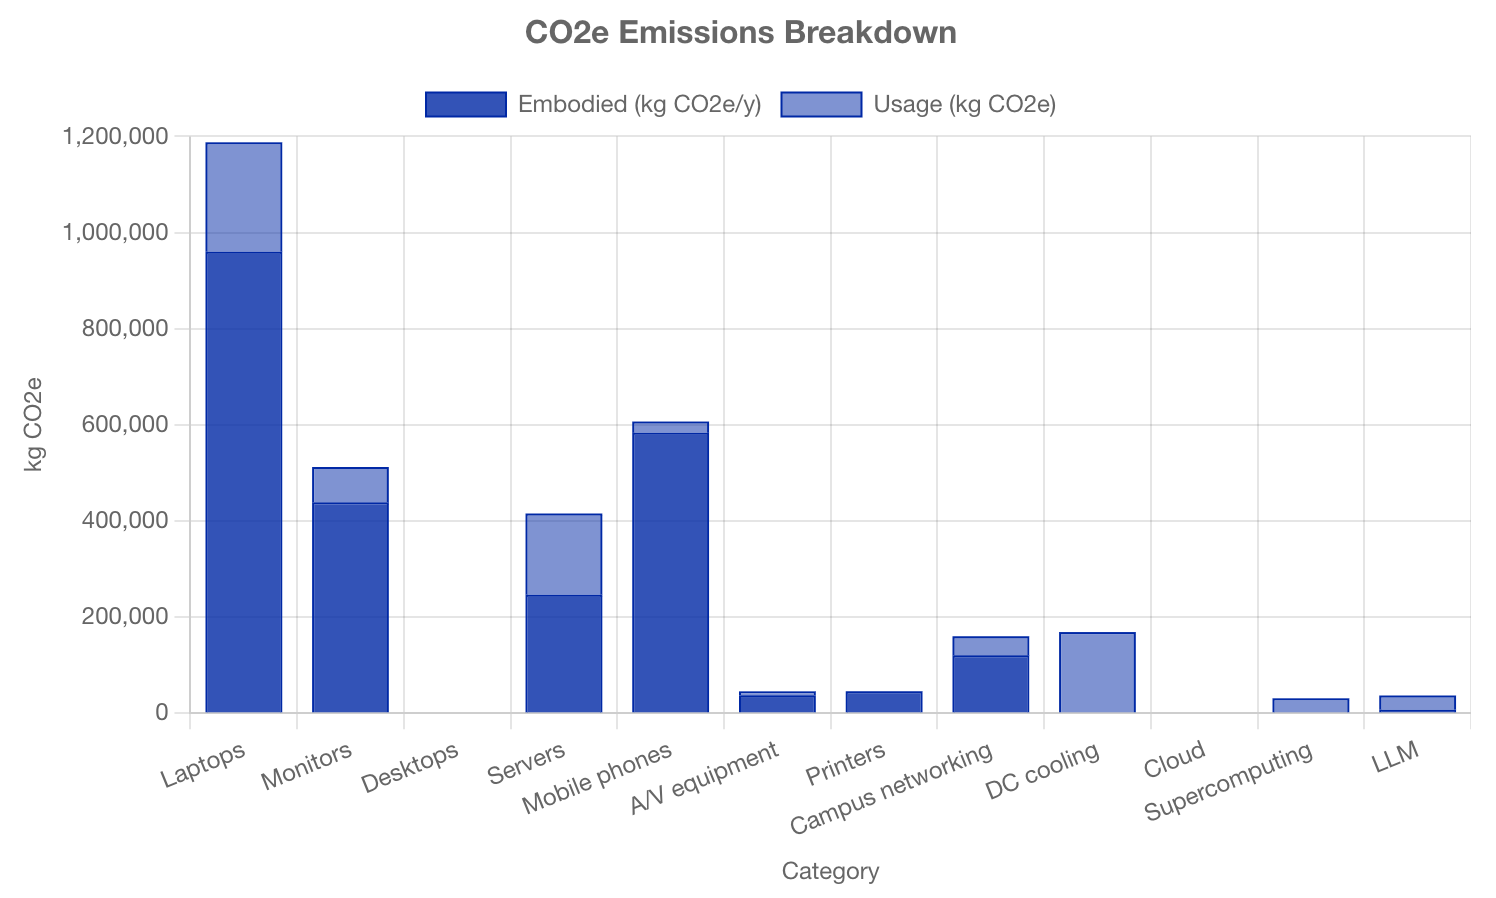
\includegraphics[width=0.8\textwidth]{fig-baseline.png}
  \caption{Baseline results}
  \label{fig:1}
\end{figure}

Many studies~\cite{wb:itu:ict,umich:factsheet} agree that a large fraction of computer and mobile phone energy demand stems from the manufacturing phase. This is due in part to the fact that such end-user devices are not used continuously. Our estimate of embodied emissions comprising approximately 85\% of total laptop emissions is near the top of the range in the literature, and it is consistent with the fact that the carbon intensity of Swiss electricity is about one quarter the EU average~\cite{electricitymaps}.

\subsubsection*{Impact of cloud computing}

Hypothetically moving all UZH server workloads from on-premise data centers to a commercial cloud provider eliminates about 170 \tcoe\ of cooling overhead, and replaces 415 \tcoe\ of total server emissions with 380 \tcoe\ of cloud emissions.

\begin{figure}[h]
  \centering
  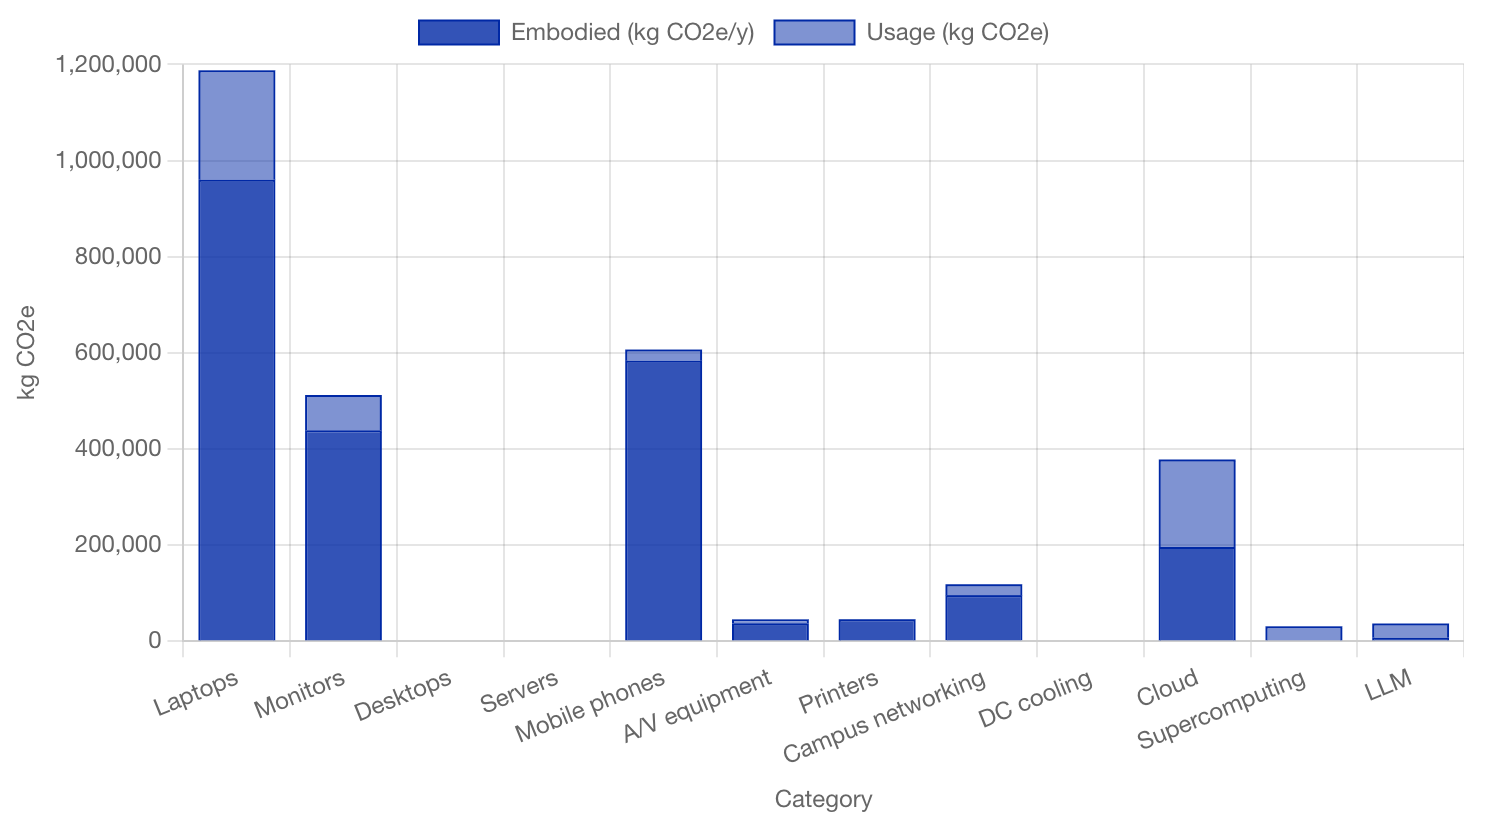
\includegraphics[width=0.8\textwidth]{fig-cloud.png}
  \caption{Migration to cloud}
  \label{fig:1}
\end{figure}

For relatively small and inefficiently cooled facilities such as those of UZH, migration to the cloud certainly improves power usage effectiveness. Whether the migration is a net win, however, depends on details that would require an in-depth engagement with the cloud provider. The results above assume a one-for-one swap of on-premise servers with cloud ones, as well as the same electricity emissions intensity for the two facilities. If the cloud footprint needed to be bigger, or if the data center were located in a region with dirtier electricity, those factors might outweight the improved cooling efficiency.

There is also a financial argument to consider: if migration to the cloud is more expensive than continued on-premise operation, the savings from not migrating might be invested in more cost effective emissions improvements (including ones not related to IT).

\subsubsection*{Impact of LLMs}

\subsection{Sensitivity analysis}
\label{sec:sensitivity:analysis}

\section{Recommendations}
\label{sec:recommendations}

Our recommendations for university policy makers can be summarized in three main points.

First, do not panic about LLMs. Their emissions comprise a small fraction of total IT emissions, they will get more efficient, and attempting to curb their use is likely to be a losing battle.

Invest in infrastructure for the long term. Run awareness campaigns and adapt IT policies so that personal devices and university IT systems are used for as long as possible. Amortize manufacturing emissions over the longest period possible.

Improve the cooling efficiency of university data centers, or engage cloud vendors and academic compute centers (such as CSCS) to validate the potential benefits of a migration to cloud.

\section{Related work}
\label{sec:related:work}



\section{Conclusion}

Our analysis shows that manufacturing (“embodied”) emissions dominate UZH's IT carbon footprint, while operational impacts, including AI adoption, are relatively modest.

\begin{itemize}

  \item Under the assumption that the vast majority (90\%) of UZH students and staff have a laptop and smartphone, manufacturing personal devices accounts for over half of UZH's IT carbon footprint. For the estimated 32,000 laptops and smartphones, embodied emissions total $\sim 2400$ \tcoe\ annually. Usage-related emissions amount to about a tenth of that.

  \item Widespread adoption of LLMs and other frontier models should have moderate impact on total emissions. If everyone at UZH made heavy use of AI (15 queries daily), this would add approximately 220 t CO2e annually, of which 160 t directly attributable to queries. While this would almost double an individual's real-time energy use, the impact on overall emissions is relatively small.

  \item Embodied emissions are an important consideration for university-owned devices as well. If we exclude personal devices and LLMs, then total IT emissions shrink to $\sim 1500$ \tcoe, of which $\frac{2}{3}$ comprises the embodied emissions of classroom computers, wall displays, printers, etc.

  \item Data center cooling and efficiency represents a potential savings opportunity. The largest operational emissions are from data center servers and cooling (320 t). UZH data centers currently require as much energy for cooling as for computation, compared to the $6-15\%$ cooling overhead of cloud industry leaders. Moving workloads to efficient cloud providers could reduce data center emissions from $\sim 560$ t to $\sim 135$ \tcoe\ annually, though this estimate requires further validation.

\end{itemize}

\printbibliography

\end{document}
